\section{Penjelasan Matplotlib}
Matplotlib adalah sebuah modul/librari Python yang menghasilkan gambar publikasi berguna untuk keperluan dalam penyajian pada data science. Matploblib juga bermutu di dalam berbagai format hardcopy dan lingkungan interaktif sepanjang platform. Matplotlib dapat digunakan di dalam script Python, shell Python dan ipython. Dengan matplotlib, kita dapat membuat sebuah plots, histograms, spectra, bar charts, errorchards, scatterplots, dan sebagainya. Pembuat matplotlib ialah seseorang yang bernama John D. Hunter yang pada 28 Agustus 2012 lalu meninggal dunia setelah bergelut dengan komplikasi kanker yang diidap beliau. Jasa beliau untuk Python Community sungguh sangat luar biasa (khususnya python untuk science [1].
       
\section{Pemasangan Matlotlib}
Disini saya menggunakan sistem operasi windows, sebelum anda menginstall matplotlib kita harus memasang python terlebih dahulu. Disini saya menggunakan python 2,7.

Jika kita sudah memasang python maka selanjutnya ialah kita memvalidasi python menggunakan CMD sampai tampilan seperti pada gambar \ref{fig:cmd}: 
\begin{figure}[!htbp]
	\centerline{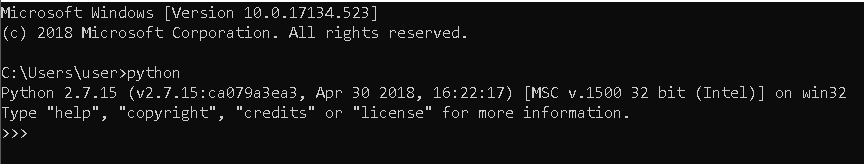
\includegraphics[width=0.85\textwidth]{figures/6/cmd.PNG}}
	\caption{Validasi Python}
	\label{fig:cmd}
\end{figure}

Jika tampilan sudah seperti gambar \ref{fig:cmd}, maka selanjutnya kita akan memasang modul matplotlib. Matplotlib dapat diinstal dengan menjalankan perintah berikut di dalam CMD, disini saya akan menggunakan pip, namun anda dapat menggunakan tool lainnya. 
\begin{figure}[!htbp]
	\centerline{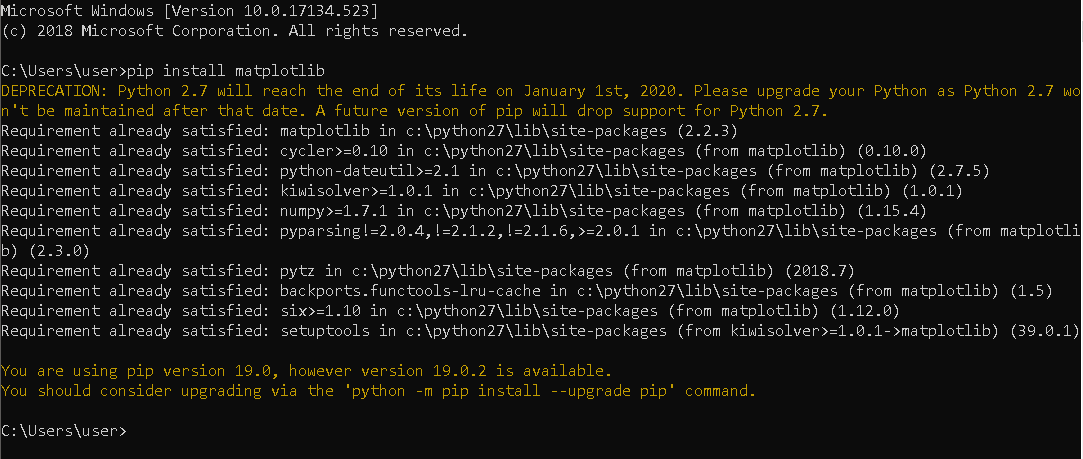
\includegraphics[width=0.85\textwidth]{figures/6/pasangmpl.PNG}}
	\caption{Pemasangan Matplotlib}
	\label{fig:pasangmpl}
\end{figure}

Jika tampilan sudah seperti gambar \ref{fig:pasangmpl}, maka matplotlib telah terpasang dan siap digunakan [2].

\section{Menggambar Plot Dasar}
Sekarang kita akan membahas tentang membuat sebuah plot dasar, atau membaca sebuah data yang berupa angka menjadi sebuah plot.
\subsection{Plot Garis}
Kita akan membahas sebuah contoh sederhana dalam menggambar sebuah plot garis menggunakan matplotlib. Dalam contoh ini, kita akan membuat sebuah garis dari data angka yang memiliki sumbu x dan y
Untuk data yang akan kita buat sebagai plot adalah sebagai berikut : 
\begin{verbatim}
x = (4,8,13,17,20)
y = (54, 67, 98, 78, 45)
\end{verbatim}

Ini dapat dilakukan dengan menggunakan seperti pada listing \ref{lst:plotgaris} : 
\lstinputlisting[caption=Skrip Plot Garis, label={lst:plotgaris}]{src/6/plotgaris.py}
Perhatikan bahwa kita menyajikan titik x dan y sebagai daftar.
Dalam contoh ini, hasilnya akan menjadi seperti pada gambar \ref{fig:plotgaris}:
\begin{figure}[!htbp]
	\centerline{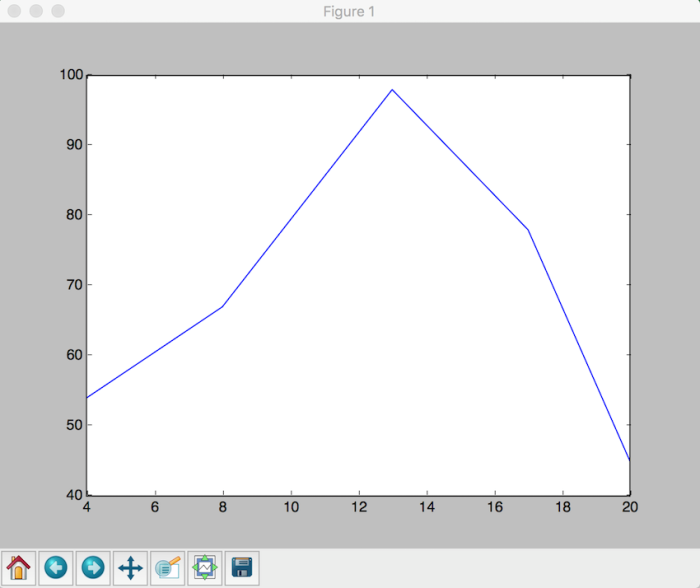
\includegraphics[width=0.85\textwidth]{figures/6/plotgaris.PNG}}
	\caption{Tampilan Plot Garis}
	\label{fig:plotgaris}
\end{figure}

Garis pada gambar di atas adalah garis default yang digambarkan untuk sebuah plot dasar, baik bentuk dan warnanya. Kita dapat memodifikasi itu dengan mengubah bentuk dan warna garis menggunakan beberapa fungsi dari dokumentasi matplotlib.

\subsection{Plot Sebaran}
Sebuah plot sebaran adalah sebuah grafik yang menunjukkan hubungan antara dua set data, di plot sebaran ini digambarkan melalui titik titik yang saling terhubung ke angka-angka yang ada di sumbu x dan y. Di dalam contoh ini, kita akan membahas menggambar sebuah plot sebaran menggunakan matplotlib.

Untuk data yang akan kita buat sebagai plot adalah sebagai berikut : 
\begin{verbatim}
x = [2,4,6,7,9,13,19,26,29,31,36,40,48,51,57,67,69,71,78,88]
y = [54,72,43,2,8,98,109,5,35,28,48,83,94,84,73,11,464,75,200,54]
\end{verbatim}
Plot sebaran dapat digambarkan menggunakan seperti pada listing \ref{lst:plotsebaran} : 
\lstinputlisting[caption=Skrip Plot Sebaran, label={lst:plotsebaran}]{src/6/plotsebaran.py}

Dalam contoh ini, hasilnya akan menjadi seperti pada gambar \ref{fig:plotsebaran}:
\begin{figure}[!htbp]
	\centerline{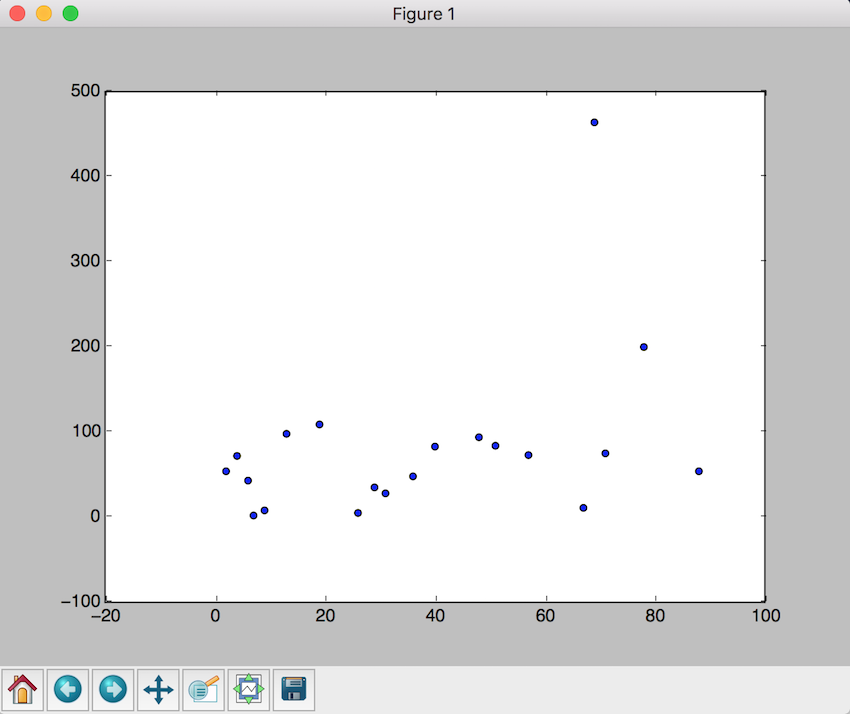
\includegraphics[width=0.85\textwidth]{figures/6/plotsebaran.PNG}}
	\caption{Tampilan Plot Sebaran}
	\label{fig:plotsebaran}
\end{figure}

Tentu saja, kita dapat mengubah warna marker sebagai tambahan untuk pengaturan lainnya, seperti yang ditunjukkan di dalam dokumentasi.

\subsection{Histogram}
Plot histogram adalah sebuah grafik yang menampilkan frekuensi data menggunakan sebuah batang, dimana angka dikelompokkan dalam rentang yang tertentu. Dengan kata lain, frekuensi setiap elemen data di dalam daftar ditunjukkan menggunakan histogram. Angka yang dikelompokkan dalam bentuk rentang tertentu. Mari lihat contoh untuk lebih mengerti ini.

Contoh data yang ingin kita tentukan histogramnya adalah sebagai berikut:
\begin{verbatim}
x = [2,4,6,5,42,543,5,3,73,64,43,97,63,76,63,8,73,97,23,45,56,89,45,3,23,2,5,78,23,56,67,78,8,3,78,34,67,23,324,234,43,544,54,33,223,443,444,234,76,432,233,23,232,242,222,221,254,222,276,300,353,354,387,364,398]
\end{verbatim}
Script Python yang dapat kita gunakan untuk menampilkan histogram seperti pada listing \ref{lst:histogram} : 
\lstinputlisting[caption=Skrip Histogram, label={lst:histogram}]{src/6/histogram.py}

Ketika kamu menjalankan script, kamu harusnya mendapatkan sesuatu serupa dengan grafik berikut (histogram) seperti pada gambar \ref{fig:histogram}:
\begin{figure}[!htbp]
	\centerline{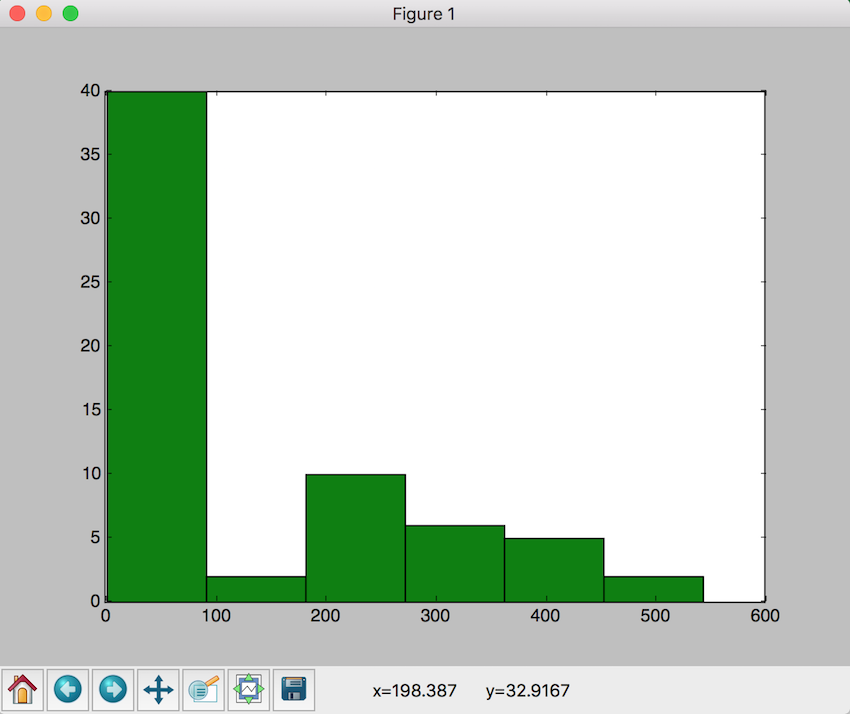
\includegraphics[width=0.85\textwidth]{figures/6/histogram.PNG}}
	\caption{Tampilan Histogram}
	\label{fig:histogram}
\end{figure}

Tentu saja ada lebih banyak parameter untuk function hist, seperti yang ditunjukkan di dokumentasi.

\subsection{Kustomisasi Plot} 
Sekarang kita dapat menambahkan judul, label untuk garis horisontal dan vertikal dengan memanggil fungsi xtitle, xlabel, dan ylabel seperti pada seperti pada listing \ref{lst:cusplot} : 
\lstinputlisting[caption=Skrip Kustomisasi Plot, label={lst:cusplot}]{src/6/cusplot.py}
Seperti pada gambar \ref{fig:cusplot}:
\begin{figure}[!htbp]
	\centerline{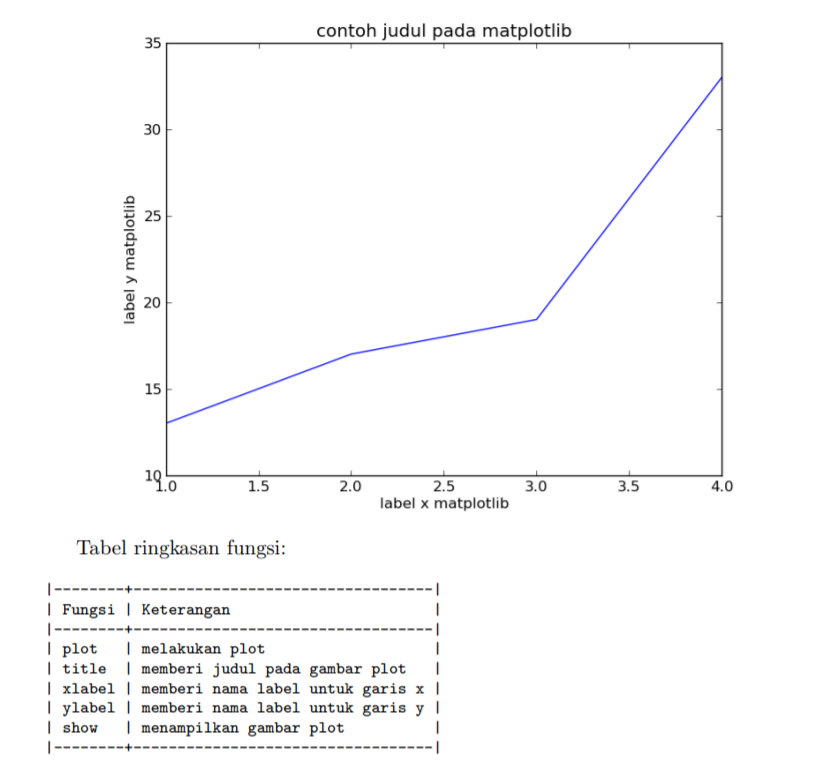
\includegraphics[width=0.85\textwidth]{figures/6/cusplot.PNG}}
	\caption{Tampilan Kustomisasi Plot}
	\label{fig:cusplot}
\end{figure}

\section{Pembacaan data dari sebuah file.txt} 
\subsection{Membuat/memasukkan data melalui notepad}
Cara yang pertama ialah dengan memasukkan seluruh data berupa angka ke sebuah halaman notepad dan kemudian disimpan sebagai file.txt (disini saya membuat nama file hasil.txt)
Seperti pada gambar \ref{fig:hasiltxt}:
\begin{figure}[!htbp]
	\centerline{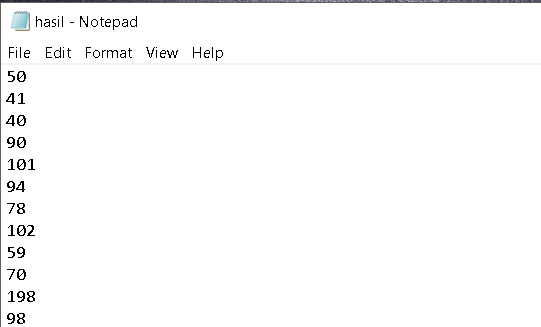
\includegraphics[width=0.85\textwidth]{figures/6/hasiltxt.PNG}}
	\caption{Data Hasil.txt}
	\label{fig:hasiltxt}
\end{figure}

\subsection{Pembacaan data}
Setelah kita berhasil membuat file dengan nama hasil.txt, kemudian kita akan memanggil file tersebut kesebuah kode program, sehingga source code seperti pada listing \ref{lst:rdata} : 
\lstinputlisting[caption=Skrip Pembacaan Data, label={lst:rdata}]{src/6/rdata.py}

Source code diatas bernama ‘ bacadata.py ‘ lalu dengan menggunakan python kita akan memanggil bacadata.py tersebut. 

Cara pemanggilan sebuah file python adalah sebagai berikut : 
\begin{enumerate}
\item Buka CMD
\item Arahkan ke direktori tempat penyimpanan file python yang kamu buat (disini saya meletakkan file python bacadata.py tersebut di desktop
\item Lalu panggil dengan perintah seperti pada gambar \ref{fig:bacadata}:
\begin{figure}[!htbp]
	\centerline{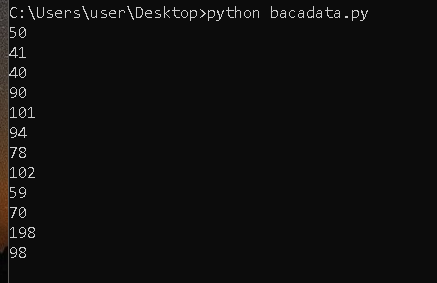
\includegraphics[width=0.85\textwidth]{figures/6/bacadata.PNG}}
	\caption{Pemanggilan bacadata.py}
	\label{fig:bacadata}
\end{figure}

\item Perlu diketahui bahwa file hasil.txt harus terletak di direktori dan folder yang sama (disini saya meletakkan hasil.txt di dekstop juga)
\item Sehingga jika python bacadata.py maka akan membaca keseluruhan isi angka pada data hasil.txt tersebut.
\item Perlu diketahui lagi bahwa ini hanya membaca dan menampilkan data berupa angka juga, sehingga hasilnya akan seperti gambar diatas.
\end{enumerate}
 
\subsection{Pemanggilan data ke sebuah plot}
Seperti pada listing \ref{lst:dataplot} : 
\lstinputlisting[caption=Skrip Pemanggilan data ke sebuah plot, label={lst:dataplot}]{src/6/dataplot.py}

Dengan menggunakan source code diatas kita bisa memanggil hasil.txt yang telah kita buat tadi ke sebuah fungsi plot, sehingga kita tidak perlu lagi menulis seluruh isi data angka di source code plot, cukup menggunakan ‘with open’ kita dapat memanggil file yang kemudian akan di baca dan ditampilkan berupa plot.

Disini saya membuat file python yang bernama panggildata.py .Sehingga jika kita panggil melalui CMD akan seperti pada gambar \ref{fig:panggildata}:
\begin{figure}[!htbp]
	\centerline{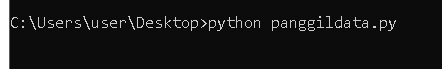
\includegraphics[width=0.85\textwidth]{figures/6/panggildata.PNG}}
	\caption{Pemanggilan panggildata.py}
	\label{fig:panggildata}
\end{figure}

Jika sudah kita panggil maka secara otomatis akan muncul figure baru seperti pada gambar \ref{fig:pplot}:
\begin{figure}[!htbp]
	\centerline{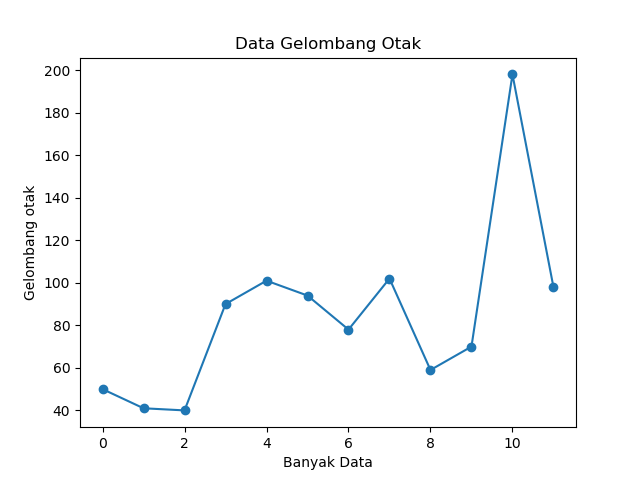
\includegraphics[width=0.85\textwidth]{figures/6/pplot.PNG}}
	\caption{Tampilan pemanggilan data ke sebuah plot}
	\label{fig:pplot}
\end{figure} 

\section{Modifikasi Hasil Plot} 
\subsection{Setting Label} 
Kita dapat Kustomisasi Tampilan pada plot, pertama kita akan membahas tentang label. Anda dapat menambahkan judul, label untuk garis horisontal dan vertikal dengan menambahkan nama label untuk garis x dan y
Disini ada contoh source code untuk menambahkan nama pada label, Seperti pada listing \ref{lst:setlabel} : 
\lstinputlisting[caption=Skrip Setting Label, label={lst:setlabel}]{src/6/setlabel.py}

Adapun hasil yang ditampilkan pada source code diatas adalah seperti pada gambar \ref{fig:setlabel}:
\begin{figure}[!htbp]
	\centerline{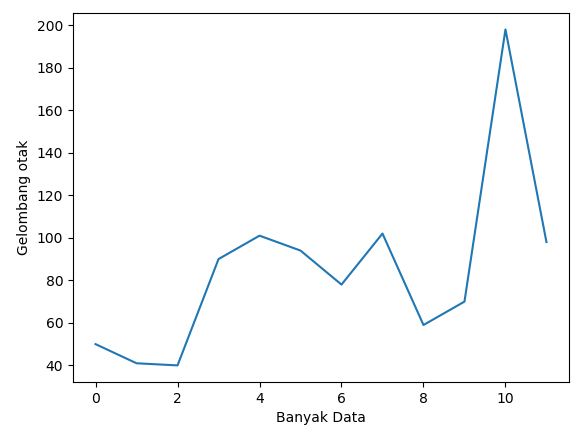
\includegraphics[width=0.85\textwidth]{figures/6/setlabel.PNG}}
	\caption{Tampilan setting label}
	\label{fig:setlabel}
\end{figure} 

Pada gambar \ref{fig:setlabel} adalah sebuat plot dengan menambahkan nama pada label x yaitu banyak data dan label y yaitu gelombang otak.

\subsection{Setting Warna}
Selanjutnya kita akan membahas bagaimana kustomisasi warna pada plot, dengan menggunakan facecolor = ‘red’ kita akan menggangi warna plot menjadi merah.

Disini ada contoh source code untuk mengganti warna pada plot, tetapi disini saya coba menggunakan plt.hist, Seperti pada listing \ref{lst:setwarna} : 
\lstinputlisting[caption=Skrip Setting Warna, label={lst:setwarna}]{src/6/setwarna.py}

Jika anda membuat source seperti diatas maka akan menampilkan hasil  seperti pada gambar \ref{fig:setwarna}:
\begin{figure}[!htbp]
	\centerline{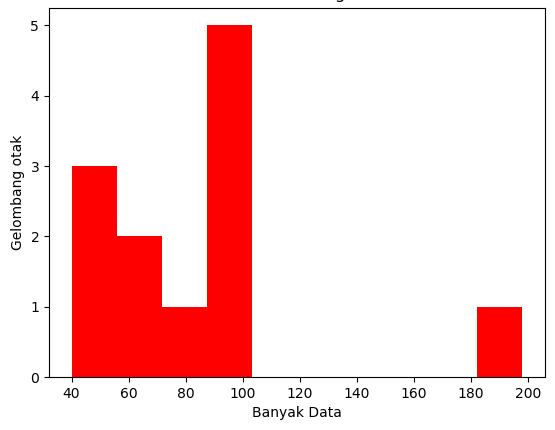
\includegraphics[width=0.85\textwidth]{figures/6/setwarna.PNG}}
	\caption{Tampilan setting warna}
	\label{fig:setwarna}
\end{figure} 

Dengan menggunakan perintah facecolor maka kita bisa mengganti warna pada plot dengan warna yang kita inginkan.

\subsection{Setting Marker}
Selanjutnya kita akan kustomisasi marker pada plot, disini kita bisa mengganti penanda label pada x dan y
Ikuti contoh source code Seperti pada listing \ref{lst:swmarker} : 
\lstinputlisting[caption=Skrip Setting Tanpa Marker, label={lst:swmarker}]{src/6/swmarker.py}

Pada source code diatas belum ada kustomisasi marker yang dibuat, lalu  hasilnya akan seperti pada gambar \ref{fig:swmarker}:
\begin{figure}[!htbp]
	\centerline{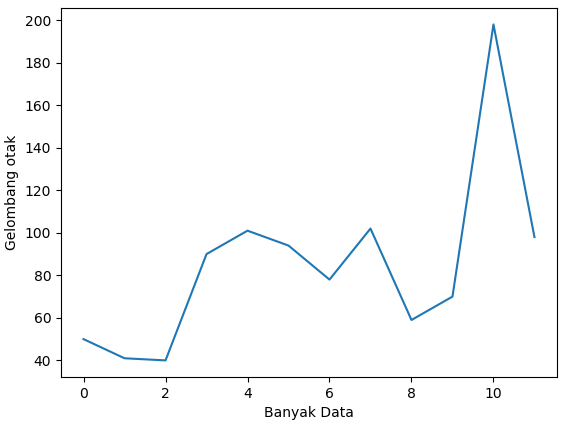
\includegraphics[width=0.85\textwidth]{figures/6/swmarker.PNG}}
	\caption{Tampilan setting tanpa marker}
	\label{fig:swmarker}
\end{figure} 

Sekarang coba kita bandingkan dengan source code berikut yang ditambahkan marker untuk kustomisasi penanda label x Seperti pada listing \ref{lst:setmarker} : 
\lstinputlisting[caption=Skrip Setting Dengan Marker, label={lst:setmarker}]{src/6/setmarker.py}
dan hasilnya akan seperti pada gambar \ref{fig:setmarker}:
\begin{figure}[!htbp]
	\centerline{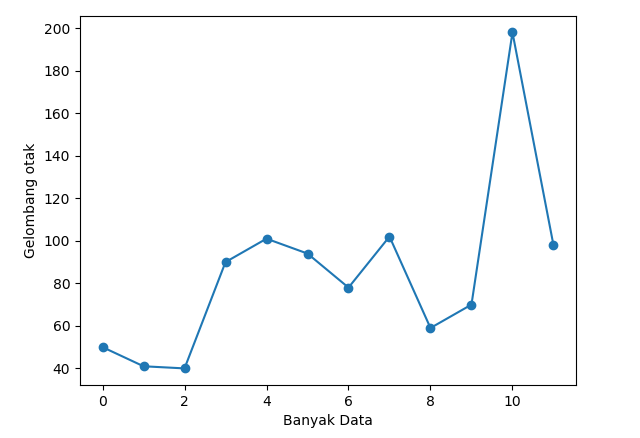
\includegraphics[width=0.85\textwidth]{figures/6/setmarker.PNG}}
	\caption{Tampilan setting dengan marker}
	\label{fig:setmarker}
\end{figure} 

Berbeda bukan sama yang gambar sebelumnya ? nah itu bisa kita kustomisasi dengan menambahkan marker pada plt.plot(x, marker='o') bisa juga o diganti dengan x dan sebagainya.

\subsection{Jenis Plot}
Pada pembahasan diawal sudah kita bahas tentang dasar-dasar plot, disini akan kita berikan hasil tampilkan pada jenis-jenis plot yang ada [4].
\begin{enumerate}
\item Plot Garis, seperti pada gambar \ref{fig:pltgaris}:
\begin{figure}[!htbp]
	\centerline{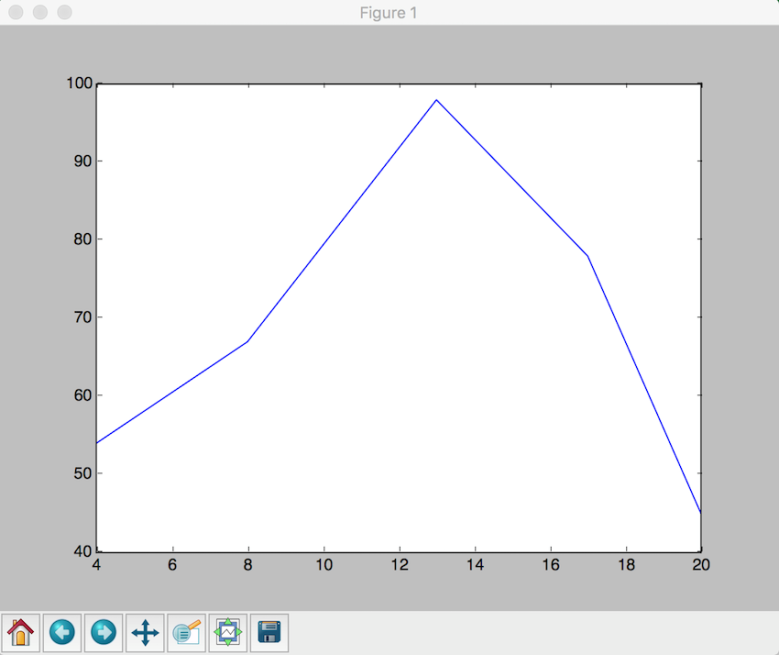
\includegraphics[width=0.85\textwidth]{figures/6/pltgaris.PNG}}
	\caption{Tampilan jenis plot garis}
	\label{fig:pltgaris}
\end{figure} 

\item Plot Sebaran, seperti pada gambar \ref{fig:pltsebaran}:
\begin{figure}[!htbp]
	\centerline{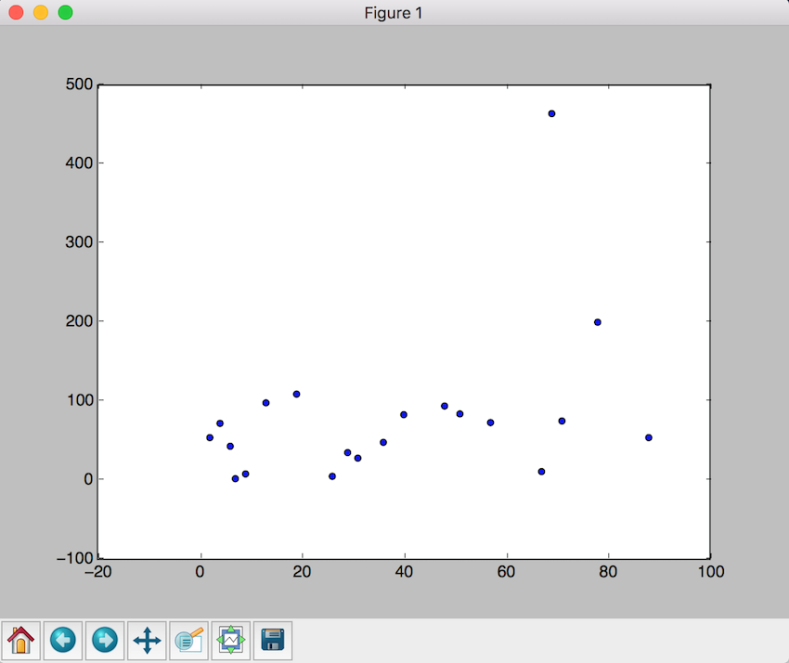
\includegraphics[width=0.85\textwidth]{figures/6/pltsebaran.PNG}}
	\caption{Tampilan jenis plot sebaran}
	\label{fig:pltsebaran}
\end{figure}

\item Histogram, seperti pada gambar \ref{fig:histogrm}:
\begin{figure}[!htbp]
	\centerline{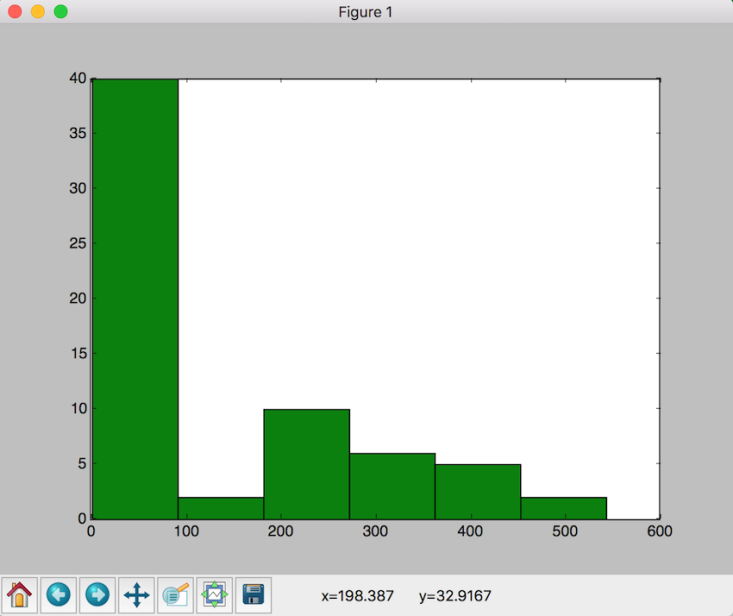
\includegraphics[width=0.85\textwidth]{figures/6/histogrm.PNG}}
	\caption{Tampilan jenis plot histogram}
	\label{fig:histogrm}
\end{figure}

\item Bar Charts, seperti pada gambar \ref{fig:barchart}:
\begin{figure}[!htbp]
	\centerline{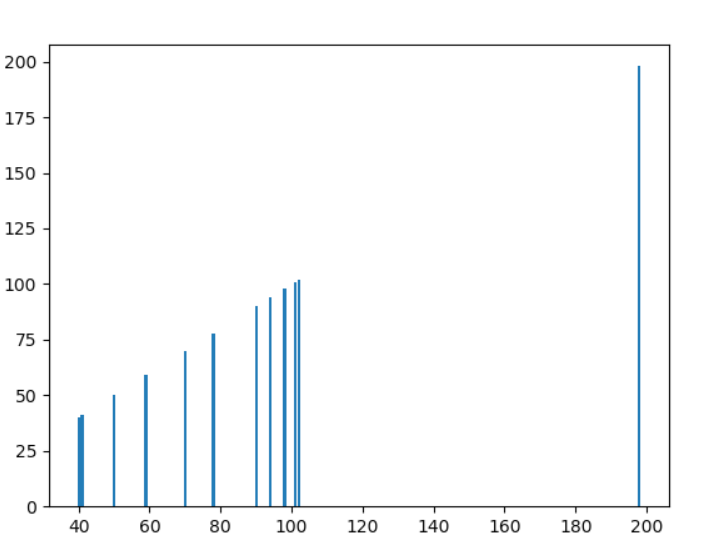
\includegraphics[width=0.85\textwidth]{figures/6/barchart.PNG}}
	\caption{Tampilan jenis plot bar charts}
	\label{fig:barchart}
\end{figure}

\item Pie, seperti pada gambar \ref{fig:pltpie}:
\begin{figure}[!htbp]
	\centerline{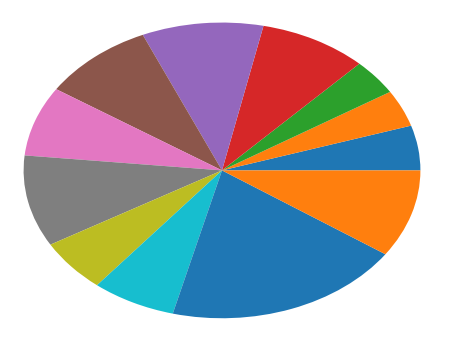
\includegraphics[width=0.85\textwidth]{figures/6/pltpie.PNG}}
	\caption{Tampilan jenis plot pie}
	\label{fig:pltpie}
\end{figure}

\item Hist, seperti pada gambar \ref{fig:hist}:
\begin{figure}[!htbp]
	\centerline{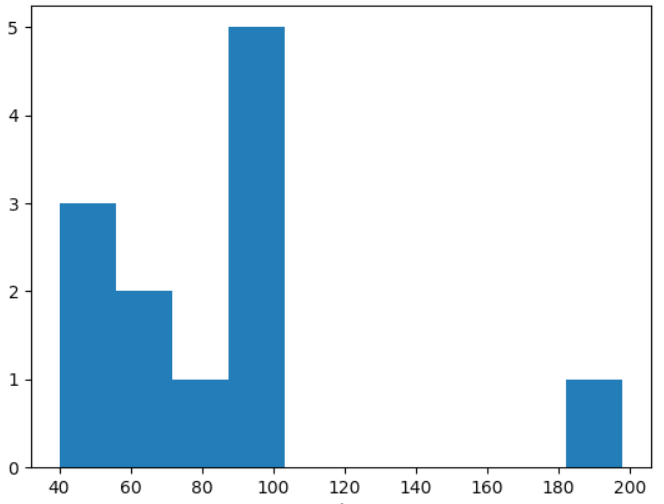
\includegraphics[width=0.85\textwidth]{figures/6/hist.PNG}}
	\caption{Tampilan jenis plot hist}
	\label{fig:hist}
\end{figure}

\item 3D Line, seperti pada gambar \ref{fig:3dline}:
\begin{figure}[!htbp]
	\centerline{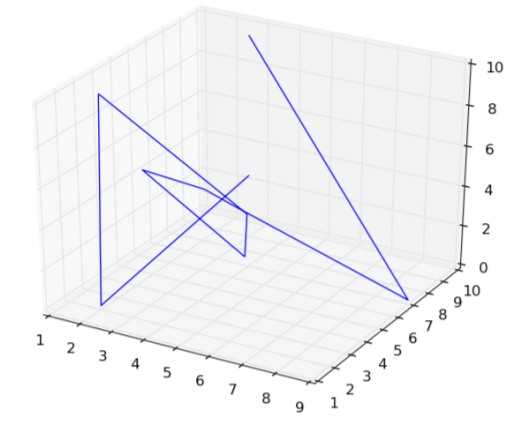
\includegraphics[width=0.85\textwidth]{figures/6/3dline.PNG}}
	\caption{Tampilan jenis plot 3D Line}
	\label{fig:3dline}
\end{figure}

\item 3D Scatter Plot, seperti pada gambar \ref{fig:3dscatter}:
\begin{figure}[!htbp]
	\centerline{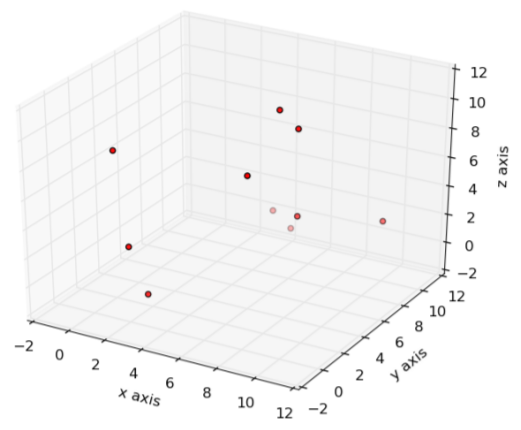
\includegraphics[width=0.85\textwidth]{figures/6/3dscatter.PNG}}
	\caption{Tampilan jenis plot 3D Scatter}
	\label{fig:3dscatter}
\end{figure}

\item 3D Bar Charts, seperti pada gambar \ref{fig:3dchart}:
\begin{figure}[!htbp]
	\centerline{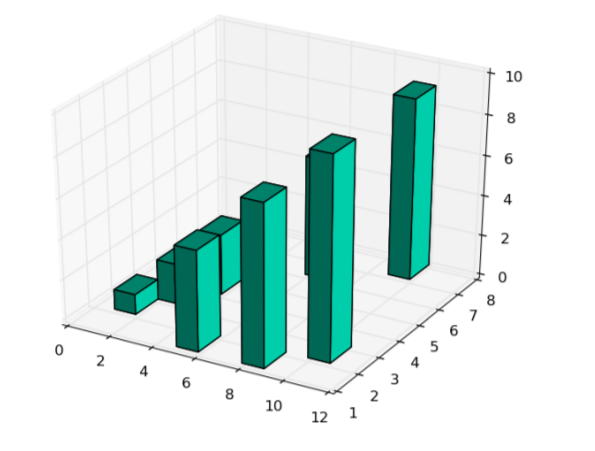
\includegraphics[width=0.85\textwidth]{figures/6/3dchart.PNG}}
	\caption{Tampilan jenis plot 3D Charts}
	\label{fig:3dchart}
\end{figure}
\end{enumerate}

\section{Plot Ditampilkan Dan Disimpan}
Sekarang kita akan membahas bagaimana cara untuk membuat plot itu bisa disimpan sebagai gambar tanpa kita panggil melalui python.
\subsection{Plot Ditampilkan}
Seperti tutorial yang sebelumnya bagaimana kita sudah mempelajari bagaimana menampilkan data menjadi sebuah plot, kita ulas kembali bagaimana caranya, dengan memanfaatkan script diawal tadi Seperti pada listing \ref{lst:showplt} : 
\lstinputlisting[caption=Skrip Plot ditampilkan, label={lst:showplt}]{src/6/showplt.py}
Hasilnya juga akan sama seperti tutorial diawal tadi seperti pada gambar \ref{fig:hasilplot}:
\begin{figure}[!htbp]
	\centerline{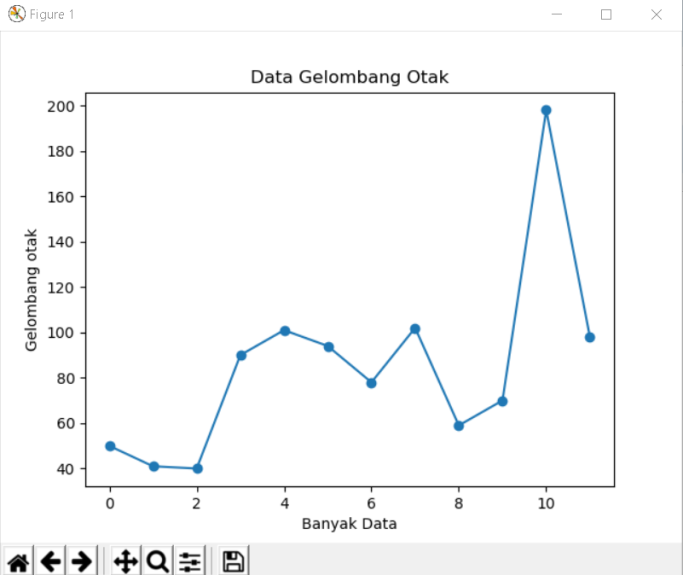
\includegraphics[width=0.85\textwidth]{figures/6/hasilplot.PNG}}
	\caption{Hasil plot ditampilkan}
	\label{fig:hasilplot}
\end{figure} 

\subsection{Plot Disimpan}
Sekarang kita akan membahas bagaimana suatu data yang sudah kita transformasi menjadi sebuah plot bisa tersimpan sebagai gambar. 
Script sama seperti Tabel 6.10 tadi, disini kita fokus ke hasil pada Gambar 6.21, ada sebuah menu dibawah hasil yang ditampilkan. 
Perhatikan gambar  \ref{fig:menuplot}:
\begin{figure}[!htbp]
	\centerline{
\includegraphics[width=0.85\textwidth]{figures/6/menuplot.PNG}}
	\caption{Menu plot disimpan}
	\label{fig:menuplot}
\end{figure} 

Dengan memanfaatkan menu save yang ada pada tampilan diatas maka secara otomatis kita bisa menyimpan hasil plot menjadi gambar ke lokasi file yang kita mau seperti pada gambar \ref{fig:prosesplot}:
\begin{figure}[!htbp]
	\centerline{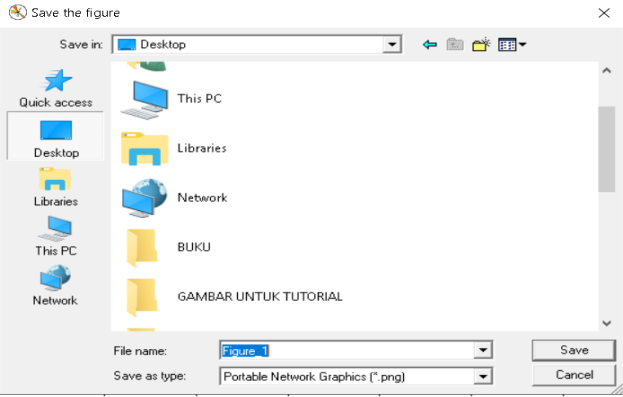
\includegraphics[width=0.85\textwidth]{figures/6/prosesplot.PNG}}
	\caption{Proses plot disimpan}
	\label{fig:prosesplot}
\end{figure} 

\section{Penanganan Error Pada Pemasangan Matlotlib}
Disini saya menggunakan sistem operasi windows, sebelum anda menginstall matplotlib kita harus memasang python terlebih dahulu. Disini saya menggunakan python 2,7.

Langsung saja kita pergi ke CMD lalu ketikan pip install matplotlib seperti pada gambar \ref{fig:errormat}:
\begin{figure}[!htbp]
	\centerline{
\includegraphics[width=0.85\textwidth]{figures/6/errormat.PNG}}
	\caption{Error Pemasangan Matplotlib}
	\label{fig:errormat}
\end{figure} 

Gambar \ref{fig:errormat} adalah tampilan error pada saat kita install matplotlib, coba anda teliti dimanakah letak error tersebut ? 
Error terletak pada sintaks ‘pip instal matplotlib‘ yang seharunya ‘pip install matplotlib’ tampaknya hanya hal kecil tapi dengan kita salah membuat sintaks maka hasil juga akan error sehingga perintah yang benar seperti pada gambar \ref{fig:pasangmat}:
\begin{figure}[!htbp]
	\centerline{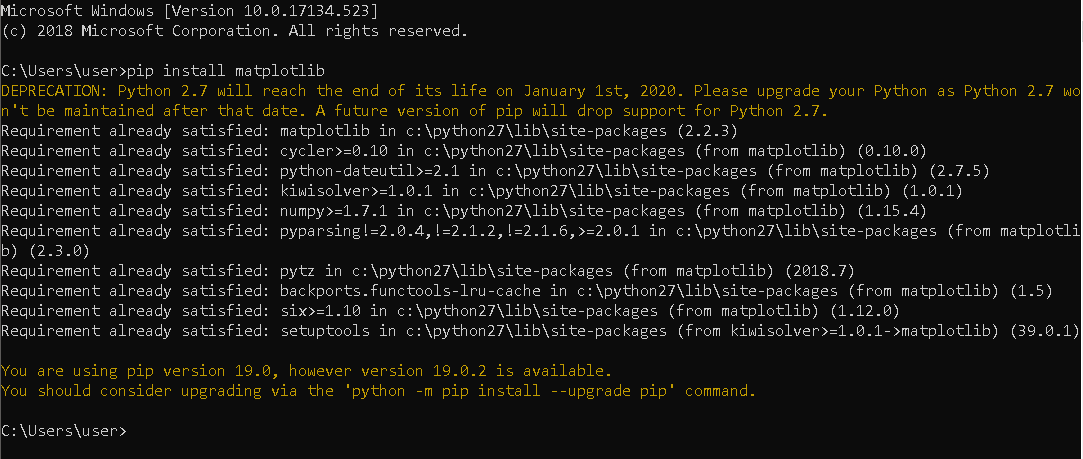
\includegraphics[width=0.85\textwidth]{figures/6/pasangmat.PNG}}
	\caption{Pemasangan Matplotlib}
	\label{fig:pasangmat}
\end{figure} 

Jika tampilan sudah seperti gambar \ref{fig:pasangmat}, maka matplotlib telah terpasang dan siap digunakan [2].

\section{Error Pada Saat Menggambar Plot Dasar}
Sekarang kita akan membahas tentang membuat sebuah plot dasar, atau membaca sebuah data yang berupa angka menjadi sebuah plot.
\subsection{Error Pada Plot Garis}
Kita akan membahas sebuah contoh sederhana dalam menggambar sebuah plot garis menggunakan matplotlib. Dalam contoh ini, kita akan membuat sebuah garis dari data angka yang memiliki sumbu x dan y.
Untuk data yang akan kita buat sebagai plot adalah sebagai berikut : 
\begin{verbatim}
x = (4,8,13,17,20)
y = (54, 67, 98, 78, 45)
\end{verbatim}
Ini dapat dilakukan dengan menggunakan script Seperti pada listing \ref{lst:pltgaris} : 
\lstinputlisting[caption=Skrip Plot Garis, label={lst:pltgaris}]{src/6/pltgaris.py}
seperti pada gambar \ref{fig:errpltgaris}:
\begin{figure}[!htbp]
	\centerline{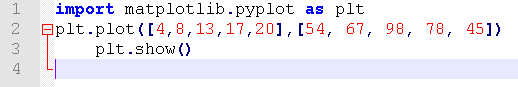
\includegraphics[width=0.85\textwidth]{figures/6/errpltgaris.PNG}}
	\caption{Skrip Error Plot Garis}
	\label{fig:errpltgaris}
\end{figure}

seperti pada gambar \ref{fig:errpltgrs}:
\begin{figure}[!htbp]
	\centerline{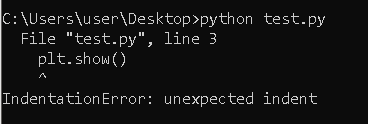
\includegraphics[width=0.85\textwidth]{figures/6/errpltgrs.PNG}}
	\caption{Error Plot Garis}
	\label{fig:errpltgrs}
\end{figure}            

Pada contoh di atas saya membuat file dengan nama test.py, dan saya panggil melalui python. Sintaks diatas adalah error karena plt.show() tidak sejajar dengan baris kedua sehingga di baca oleh program plt.show() itu adalah turunan dari baris kedua, sehingga solusinya seperti pada gambar \ref{fig:solepg}:
\begin{figure}[!htbp]
	\centerline{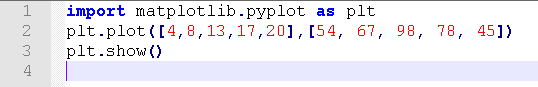
\includegraphics[width=0.85\textwidth]{figures/6/solepg.PNG}}
	\caption{Solusi Error Plot Garis}
	\label{fig:solepg}
\end{figure}            

Dan jika dipanggil melalui python hasilnya akan seperti pada gambar \ref{fig:erpg}:
\begin{figure}[!htbp]
	\centerline{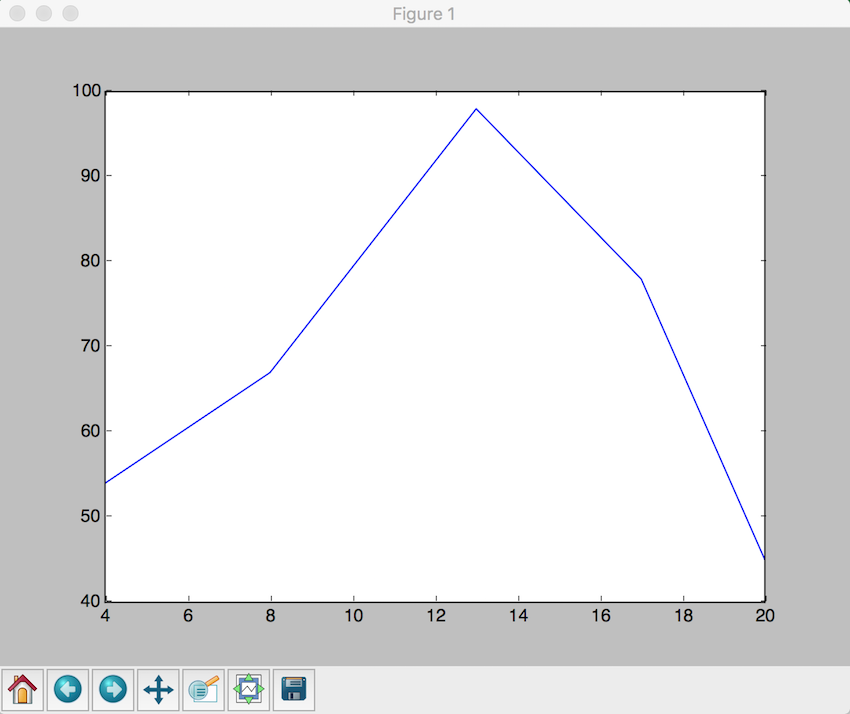
\includegraphics[width=0.85\textwidth]{figures/6/erpg.PNG}}
	\caption{Error Plot Garis}
	\label{fig:erpg}
\end{figure}       

Gambar \ref{fig:erpg} adalah error kedua pada program plot garis, disini errornya adalah kita tidak meletakkan koma di antara sumbu x dan y, bisa kita temui di 
plt.plot([4,8,13,17,20] [54, 67, 98, 78, 45]) yang seharusnya seperti pada gambar \ref{fig:solpg}:
\begin{figure}[!htbp]
	\centerline{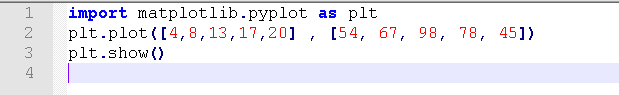
\includegraphics[width=0.85\textwidth]{figures/6/solpg.PNG}}
	\caption{Solusi Error Plot Garis}
	\label{fig:solpg}
\end{figure}       

\subsection{Plot Sebaran}
Sebuah plot sebaran adalah sebuah grafik yang menunjukkan hubungan antara dua set data, di plot sebaran ini digambarkan melalui titik titik yang saling terhubung ke angka-angka yang ada di sumbu x dan y. Di dalam contoh ini, kita akan membahas menggambar sebuah plot sebaran menggunakan matplotlib.

Untuk data yang akan kita buat sebagai plot adalah sebagai berikut : 
\begin{verbatim}
x = [2,4,6,7,9,13,19,26,29,31,36,40,48,51,57,67,69,71,78,88]
y = [54,72,43,2,8,98,109,5,35,28,48,83,94,84,73,11,464,75,200,54]
\end{verbatim}
Plot sebaran dapat digambarkan menggunakan script Seperti pada listing \ref{lst:pltsebaran} : 
\lstinputlisting[caption=Skrip Plot Sebaran, label={lst:pltsebaran}]{src/6/pltsebaran.py}

Masalah atau error yang biasa timbul adalah seperti pada gambar \ref{fig:errpltsebaran}:
\begin{figure}[!htbp]
	\centerline{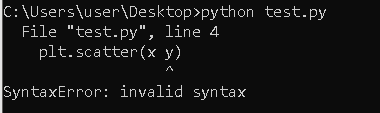
\includegraphics[width=0.85\textwidth]{figures/6/errpltsebaran.PNG}}
	\caption{Error Plot Sebaran}
	\label{fig:errpltsebaran}
\end{figure}       

Solusinya adalah dengan menambahkan koma di antara x dan y (x,y)
Atau seperti pada gambar \ref{fig:soleps}:
\begin{figure}[!htbp]
	\centerline{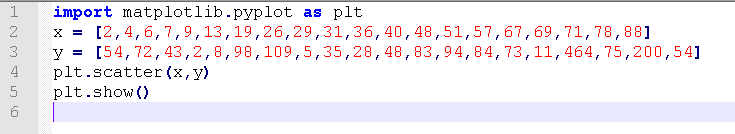
\includegraphics[width=0.85\textwidth]{figures/6/soleps.PNG}}
	\caption{Solusi Error Plot Sebaran}
	\label{fig:soleps}
\end{figure}      

Dalam contoh lain error bisa menjadi seperti pada gambar \ref{fig:errpltseb}:
\begin{figure}[!htbp]
	\centerline{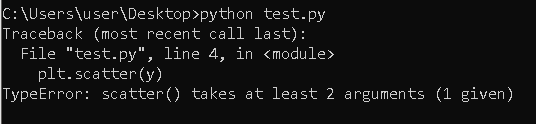
\includegraphics[width=0.85\textwidth]{figures/6/errpltseb.PNG}}
	\caption{Error Plot Sebaran}
	\label{fig:errpltseb}
\end{figure}       

Solusinya adalah terdapat pada plt.scatter(y) yang seharunya menjadi  plt.scatter(x,y) karena tidak mungkin kita mau menampilkan gambar yang sudah kita defenisikan x dan y tetapi kita hanya menampilkan 1 sumbu saja,
Dalam contoh ini, hasilnya akan menjadi seperti pada gambar \ref{fig:solepsb}:
\begin{figure}[!htbp]
	\centerline{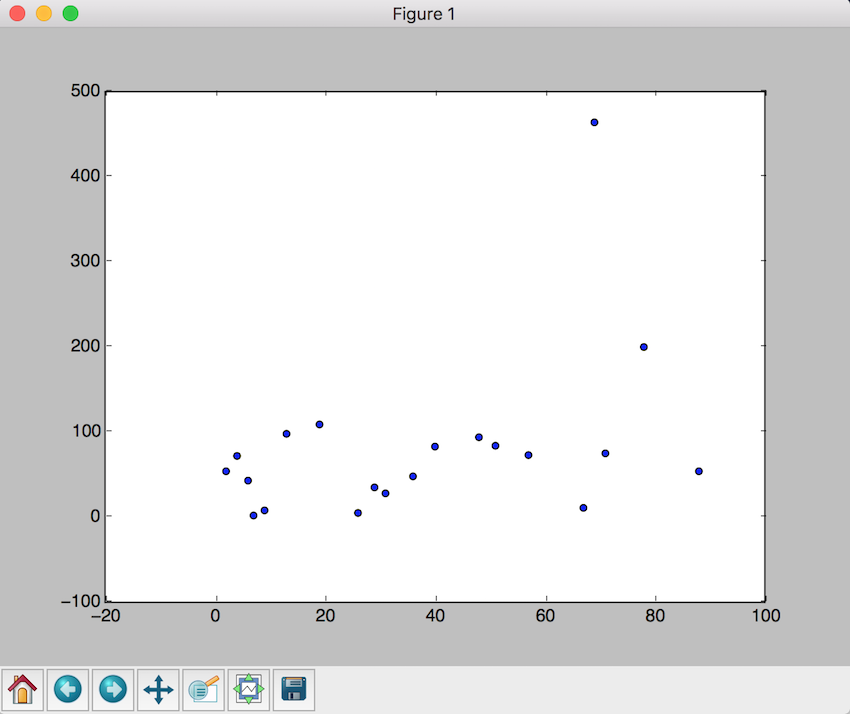
\includegraphics[width=0.85\textwidth]{figures/6/solepsb.PNG}}
	\caption{Solusi Error Plot Sebaran}
	\label{fig:solepsb}
\end{figure}      

\subsection{Error Pada Histogram}
Plot histogram adalah sebuah grafik yang menampilkan frekuensi data menggunakan sebuah batang, dimana angka dikelompokkan dalam rentang yang tertentu. Dengan kata lain, frekuensi setiap elemen data di dalam daftar ditunjukkan menggunakan histogram. Angka yang dikelompokkan dalam bentuk rentang tertentu. Mari lihat contoh untuk lebih mengerti ini.
Contoh data yang ingin kita tentukan histogramnya adalah sebagai berikut:
\verb|x = [2,4,6,5,42,543,5,3,73,64,43,97,63,76,63,8,73,97,23,45,56,89,45,3,23,2,5,78,23,56,67,78,8,3,78,34,67,23,324,234,43,544,54,33,223,443,444,234,76,432,233,23,232,242,222,221,254,222,276,300,353,354,387,364,398]|
Script Python yang dapat kita gunakan untuk menampilkan histogram pada data di atas adalah Seperti pada listing \ref{lst:histogrm} : 
\lstinputlisting[caption=Skrip Histogram, label={lst:histogrm}]{src/6/histogrm.py}

Error yang biasa ditemukan adalah seperti pada gambar \ref{fig:errhisto}:
\begin{figure}[!htbp]
	\centerline{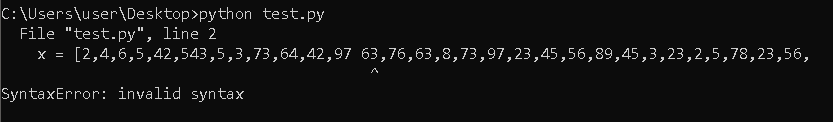
\includegraphics[width=0.85\textwidth]{figures/6/errhisto.PNG}}
	\caption{Error Histogram}
	\label{fig:errhisto}
\end{figure}       

Solusi untuk error diatas adalah pada saat mengetik script ada yang terlewat tanpa memberikan koma setelah angka, disini kita lupa memberi koma pada 97 dan 63. Seharusnya seperti pada gambar \ref{fig:solhisto}:
\begin{figure}[!htbp]
	\centerline{
\includegraphics[width=0.85\textwidth]{figures/6/solhisto.PNG}}
	\caption{Solusi Error Histogram}
	\label{fig:solhisto}
\end{figure}      

Kalau dari error yanglain adalah kita sebagai orang indonesia yang masih awam dengan sebutan warna atau color untuk program, tanpa sengaja kita mendefenisikan color=hijau. Itu jelas salah karena komputer atau program tidak akan mengerti bahasa itu, disini dapat kita ubah dengan facecolor = ‘green’ atau seperti pada gambar \ref{fig:solhistogrm}:
\begin{figure}[!htbp]
	\centerline{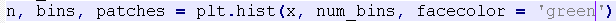
\includegraphics[width=0.85\textwidth]{figures/6/solhistogrm.PNG}}
	\caption{Solusi Error Histogram}
	\label{fig:solhistogrm}
\end{figure}      

Hasil tampilannya seperti pada gambar \ref{fig:showhisto}:
\begin{figure}[!htbp]
	\centerline{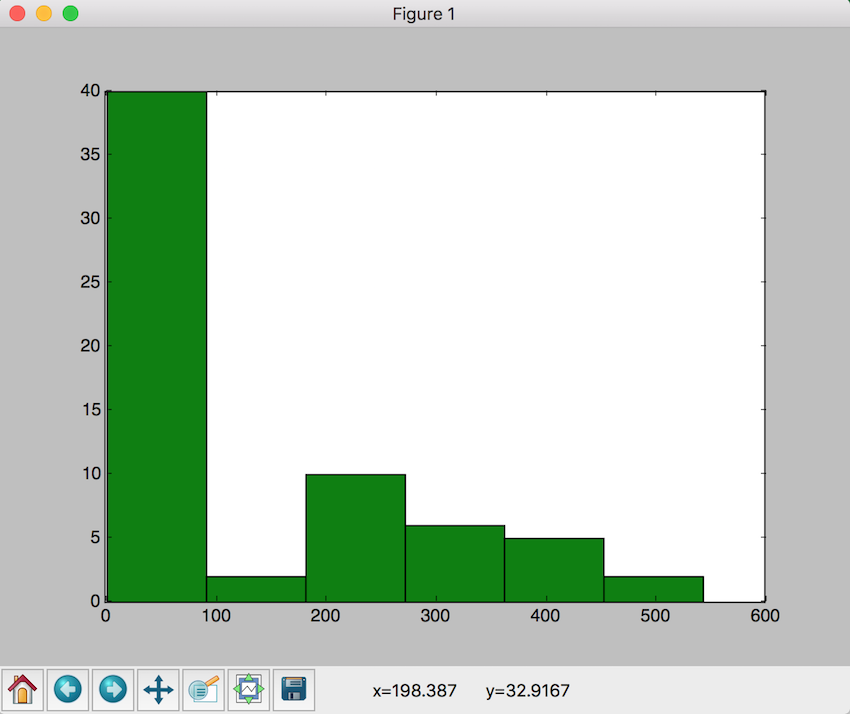
\includegraphics[width=0.85\textwidth]{figures/6/showhisto.PNG}}
	\caption{Tampilan Histogram}
	\label{fig:showhisto}
\end{figure} 

\subsection{Error Pada Saat Kustomisasi Plot} 
Sekarang kita dapat menambahkan judul, label untuk garis horisontal dan vertikal dengan memanggil fungsi xtitle, xlabel, dan ylabel Seperti pada listing \ref{lst:cuserrplt} : 
\lstinputlisting[caption=Kustomisasi Plot, label={lst:cuserrplt}]{src/6/cuserrplt.py}
Pada script diatas sudah ada fungsi title, xlabel dan ylabel.Tetapi ada beberapa error yang mungkin didapat jika kita salah pada pengetikan, seperti pada gambar \ref{fig:errcusplot}:
\begin{figure}[!htbp]
	\centerline{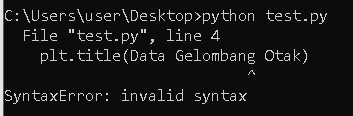
\includegraphics[width=0.85\textwidth]{figures/6/errcusplot.PNG}}
	\caption{Error Kustomisasi Plot}
	\label{fig:errcusplot}
\end{figure}       

Solusi dari error diatas adalah dengan menambahkan tanda kutip pada setiap kita mendefenisikan title, sehingga seperti pada gambar \ref{fig:solcusplot}:
\begin{figure}[!htbp]
	\centerline{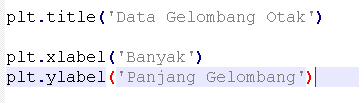
\includegraphics[width=0.85\textwidth]{figures/6/solcusplot.PNG}}
	\caption{Solusi Error Kustomisasi Plot}
	\label{fig:solcusplot}
\end{figure}      

seperti pada gambar \ref{fig:errcusplt}:
\begin{figure}[!htbp]
	\centerline{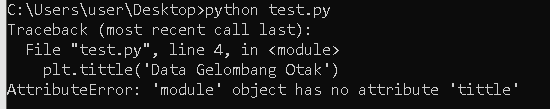
\includegraphics[width=0.85\textwidth]{figures/6/errcusplt.PNG}}
	\caption{Error Kustomisasi Plot}
	\label{fig:errcusplt}
\end{figure}
Error \ref{fig:errcusplt} adalah kesalahan penulisan pada fungsi plt.tittle yang seharusnya digunakan plt.title (tanpa double T) atau seperti pada gambar \ref{fig:solcp}:
\begin{figure}[!htbp]
	\centerline{
\includegraphics[width=0.85\textwidth]{figures/6/solcp.PNG}}
	\caption{Solusi Error Kustomisasi Plot}
	\label{fig:solcp}
\end{figure}

Hasil tampilannya seperti pada gambar \ref{fig:showcp}:
\begin{figure}[!htbp]
	\centerline{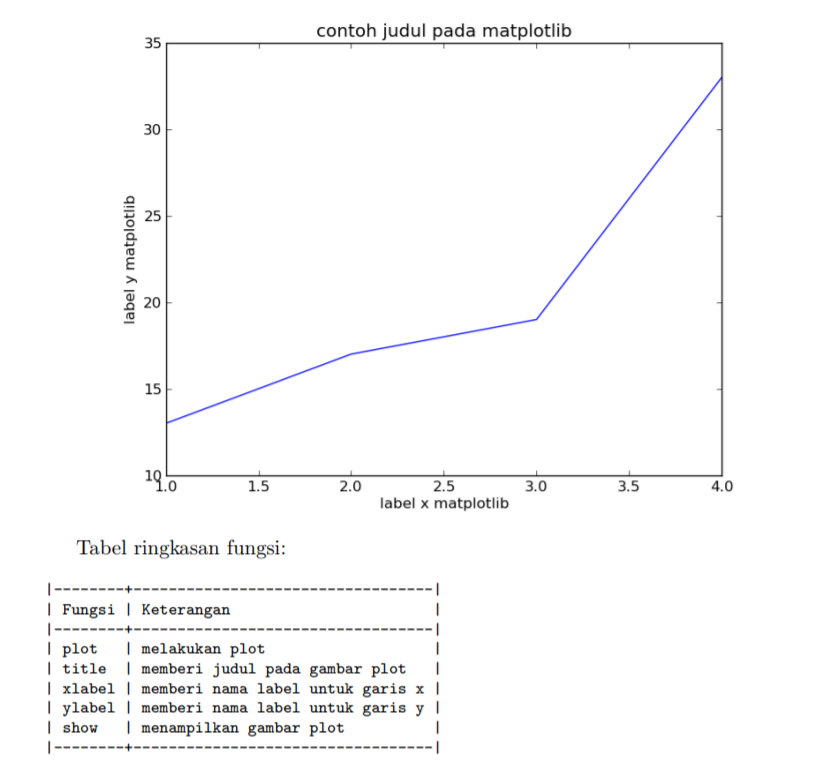
\includegraphics[width=0.85\textwidth]{figures/6/showcp.PNG}}
	\caption{Tampilan Kustomisasi Plot}
	\label{fig:showcp}
\end{figure} 

\section{Error Pada Pembacaan data dari sebuah file.txt} 
\subsection{Membuat/memasukkan data melalui notepad}
Cara yang pertama ialah dengan memasukkan seluruh data berupa angka ke sebuah halaman notepad dan kemudian disimpan sebagai file.txt (disini saya membuat nama file hasil.txt) seperti pada gambar \ref{fig:datahasil}:
\begin{figure}[!htbp]
	\centerline{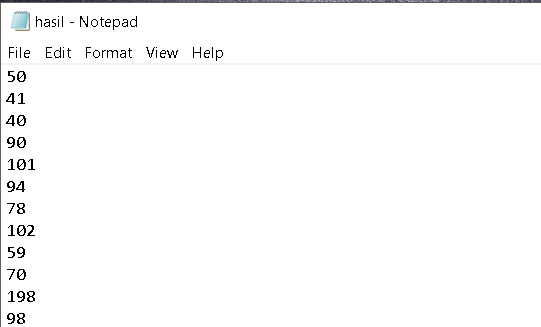
\includegraphics[width=0.85\textwidth]{figures/6/datahasil.PNG}}
	\caption{Data Hasil.txt}
	\label{fig:datahasil}
\end{figure} 

\subsection{Error Pada Pembacaan data}
Setelah kita berhasil membuat file dengan nama hasil.txt, kemudian kita akan memanggil file tersebut kesebuah kode program, sehingga source code akan Seperti pada listing \ref{lst:rdt} : 
\lstinputlisting[caption=Skrip Pembacaan data, label={lst:rdt}]{src/6/rdt.py}

Source code diatas bernama ‘ bacadata.py ‘ lalu dengan menggunakan python kita akan memanggil bacadata.py tersebut. 
Cara pemanggilan sebuah file python adalah sebagai berikut :
\begin{enumerate} 
\item Buka CMD
\item Arahkan ke direktori tempat penyimpanan file python yang kamu buat (disini saya meletakkan file python bacadata.py tersebut di desktop
\item Lalu panggil dengan perintah berikut seperti pada gambar \ref{fig:panggilbcdt}:
\begin{figure}[!htbp]
	\centerline{
\includegraphics[width=0.85\textwidth]{figures/6/panggilbcdt.PNG}}
	\caption{Panggil File bacadata.py}
	\label{fig:panggilbcdt}
\end{figure} 
Adapun error-error pada script diatas ialah seperti pada gambar \ref{fig:errdata}:
\begin{figure}[!htbp]
	\centerline{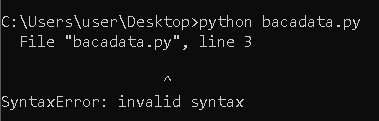
\includegraphics[width=0.85\textwidth]{figures/6/errdata.PNG}}
	\caption{Error pada pembacaan data}
	\label{fig:errdata}
\end{figure} 

Error diatas didapatkan dari script dibawah ini  seperti pada gambar \ref{fig:lsterrdata}:
\begin{figure}[!htbp]
	\centerline{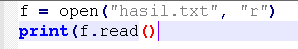
\includegraphics[width=0.85\textwidth]{figures/6/lsterrdata.PNG}}
	\caption{Script Error pada pembacaan data}
	\label{fig:lsterrdata}
\end{figure} 

Yang membedakan script diatas dengan script diawal iyalah kita secara tidak sengaja lupa memberi kurung penutup pada script diatas, sehingga solusinya ialah seperti pada gambar \ref{fig:solerrdata}:
\begin{figure}[!htbp]
	\centerline{\includegraphics[width=0.85\textwidth]{figures/6/solerrdata.PNG}}
	\caption{Solusi Error pada pembacaan data}
	\label{fig:solerrdata}
\end{figure} 

Adapun hasil dari script pada pembacaan data diatas ialah seperti pada gambar \ref{fig:showdata}:
\begin{figure}[!htbp]
	\centerline{\includegraphics[width=0.85\textwidth]{figures/6/showdata.PNG}}
	\caption{Tampilan pada pembacaan data}
	\label{fig:showdata}
\end{figure} 
\end{enumerate}

\subsection{Error Pemanggilan data ke sebuah plot}
Seperti pada listing \ref{lst:panggildp} : 
\lstinputlisting[caption=Skrip pemanggilan data ke sebuah plot, label={lst:rdt}]{src/6/panggildp.py}

Pada script diatas kita akan memanggil atau membaca file yang telah kita buat tadi yang bernama hasil.txt, tetapi biasa terdapat error-error pada script tersebut yaitu seperti pada gambar \ref{fig:errpd}:
\begin{figure}[!htbp]
	\centerline{\includegraphics[width=0.85\textwidth]{figures/6/errpd.PNG}}
	\caption{Error pemanggilan data}
	\label{fig:errpd}
\end{figure} 

Error pada gambar diatas terdapat pada x.append(int(row[1])) disini artinya kita membaca data pada baris kedua, jika [0] maka baris pertama dan [2] maka baris kedua dan seterusnya. Itulah yang menyebabkan script bisa jadi error, sehingga solusi nya adalah mengganti angka 1 dengan 0 seperti pada gambar \ref{fig:solepd}:
\begin{figure}[!htbp]
	\centerline{\includegraphics[width=0.85\textwidth]{figures/6/solepd.PNG}}
	\caption{Solusi Error pemanggilan data}
	\label{fig:solepd}
\end{figure} 

Error lainnya seperti pada gambar \ref{fig:epd}:
\begin{figure}[!htbp]
	\centerline{\includegraphics[width=0.85\textwidth]{figures/6/epd.PNG}}
	\caption{Error pemanggilan data}
	\label{fig:epd}
\end{figure} 

Pada gambar diatas coba kita teliti kembali pada script yang diawal,  for row in plots, seharusnya setelah itu kita tambahkan ‘:’ agar tidak error seperti pada gambar \ref{fig:sepd}:
\begin{figure}[!htbp]
	\centerline{\includegraphics[width=0.85\textwidth]{figures/6/sepd.PNG}}
	\caption{Solusi Error pemanggilan data}
	\label{fig:sepd}
\end{figure} 
  
Error lainnya seperti pada gambar \ref{fig:etpd}:
\begin{figure}[!htbp]
	\centerline{\includegraphics[width=0.85\textwidth]{figures/6/etpd.PNG}}
	\caption{Error tampilan  pemanggilan data}
	\label{fig:etpd}
\end{figure} 

Pada gambar diatas didapatkan dari script berikut Seperti pada listing \ref{lst:etpd} : 
\lstinputlisting[caption=Contoh Skrip error pemanggilan data ke sebuah plot, label={lst:etpd}]{src/6/etpd.py}

Namun kenapa masih kosong tanpa ada gambaran sebuah plot ? Itu karena kita tidak meletakkan sumbu yang ingin dibaca oleh program, yaitu sumbu x, error terdapat pada baris ke 13, yang seharusnya seperti pada gambar \ref{fig:solerrpd}:
\begin{figure}[!htbp]
	\centerline{\includegraphics[width=0.85\textwidth]{figures/6/solerrpd.PNG}}
	\caption{Solusi Error pemanggilan data}
	\label{fig:solerrpd}
\end{figure} 

Error lainnya seperti pada gambar \ref{fig:errpdl}:
\begin{figure}[!htbp]
	\centerline{\includegraphics[width=0.85\textwidth]{figures/6/errpdl.PNG}}
	\caption{Error pemanggilan data}
	\label{fig:errpdl}
\end{figure} 

Adapun error diatas karena kita mengganti marker menjadi A dan tidak bisa di pahami oleh program,adapun marker yang bisa kita buat pada matplotlib yaitu seperti pada gambar \ref{fig:markermat}:
\begin{figure}[!htbp]
	\centerline{\includegraphics[width=0.85\textwidth]{figures/6/markermat.PNG}}
	\caption{Marker Pada Matplotlib}
	\label{fig:markermat}
\end{figure} 

Sekarang contoh jika kita ingin mengubah marker menjadi square yaitu seperti pada gambar \ref{fig:lstmar}:
\begin{figure}[!htbp]
	\centerline{\includegraphics[width=0.85\textwidth]{figures/6/lstmar.PNG}}
	\caption{Skrip Marker Pada Matplotlib}
	\label{fig:lstmar}
\end{figure} 

Adapun hasil dari script diatas jika mengubah marker menjadi s ialah seperti pada gambar \ref{fig:solem}:
\begin{figure}[!htbp]
	\centerline{\includegraphics[width=0.85\textwidth]{figures/6/solem.PNG}}
	\caption{Solusi Error Marker}
	\label{fig:solem}
\end{figure}  

\section{Error Pada Modifikasi Hasil Plot}
\subsection{Error Setting Label} 
Kita dapat Kustomisasi Tampilan pada plot, pertama kita akan membahas tentang label. Anda dapat menambahkan judul, label untuk garis horisontal dan vertikal dengan menambahkan nama label untuk garis x dan y
Disini ada contoh source code untuk menambahkan nama pada label, Seperti pada listing \ref{lst:settlbl} : 
\lstinputlisting[caption=Skrip Setting Label, label={lst:settlbl}]{src/6/settlbl.py}

Pada script diatas kita dapat mengubah kalimat yang terdapat pada xlabel dan ylabel. 
Tetapi setidaknya ada beberapa error yang biasa dialami pada script diatas yaitu seperti pada gambar \ref{fig:errsetlbl}:
\begin{figure}[!htbp]
	\centerline{\includegraphics[width=0.85\textwidth]{figures/6/errsetlbl.PNG}}
	\caption{Error Setting Label}
	\label{fig:errsetlbl}
\end{figure}  

Seperti yang error sebelumnya juga, kita secara tidak sengaja lupa memberi tanda kutip pada xlabel dan ylabel sehingga solusinya adalah seperti pada gambar \ref{fig:solesl}:
\begin{figure}[!htbp]
	\centerline{\includegraphics[width=0.85\textwidth]{figures/6/solesl.PNG}}
	\caption{Solusi Error Setting Label}
	\label{fig:solesl}
\end{figure}  

Adapun hasil dari setting label adalah seperti pada gambar \ref{fig:showtsesl}:
\begin{figure}[!htbp]
	\centerline{\includegraphics[width=0.85\textwidth]{figures/6/showtsesl.PNG}}
	\caption{Tampilan Solusi Error Setting Label}
	\label{fig:showtsesl}
\end{figure}   
Yang bertanda merah ialah xlabel dan ylabel yang telahdi setting

Adapun hasil yang ditampilkan pada source code diatas adalah seperti pada gambar \ref{fig:showsl}:
\begin{figure}[!htbp]
	\centerline{\includegraphics[width=0.85\textwidth]{figures/6/showsl.PNG}}
	\caption{Tampilan Setting Label}
	\label{fig:showsl}
\end{figure}   

\subsection{Error Setting Warna}
Selanjutnya kita akan membahas bagaimana kustomisasi warna pada plot, dengan menggunakan facecolor = ‘red’ kita akan menggangi warna plot menjadi merah.

Disini ada contoh source code untuk mengganti warna pada plot, tetapi disini saya coba menggunakan plt.hist, Seperti pada listing \ref{lst:settwarna} : 
\lstinputlisting[caption=Skrip setting warna, label={lst:settwarna}]{src/6/settwarna.py}

Pada script diatas kita akan mengubah color atau warna pada plot hist yang akan kita baca dari data hasil.txt, tetapi ada beberapa error yang di dapat sebelum script diatas dibuat seperti pada gambar \ref{fig:errsetwar}:
\begin{figure}[!htbp]
	\centerline{\includegraphics[width=0.85\textwidth]{figures/6/errsetwar.PNG}}
	\caption{Error Setting Warna}
	\label{fig:errsetwar}
\end{figure}   

Pada gambar diatas kita salah memberikan warna pada facecolor yang scriptnya seperti pada gambar \ref{fig:solesw}:
\begin{figure}[!htbp]
	\centerline{\includegraphics[width=0.85\textwidth]{figures/6/solesw.PNG}}
	\caption{Solusi Error Setting Warna}
	\label{fig:solesw}
\end{figure}   

Python tidak memahami pendefenisian merah untuk facecolor, adapun kurang lebih modul color pada matplotlib adalah seperti pada gambar \ref{fig:wsa}:
\begin{figure}[!htbp]
	\centerline{\includegraphics[width=0.85\textwidth]{figures/6/wti.PNG}}
	\caption{Color Pada Matplotlib 3}
	\label{fig:wti}
\end{figure}   

\begin{figure}[!htbp]
	\centerline{\includegraphics[width=0.85\textwidth]{figures/6/wdu.PNG}}
	\caption{Color Pada Matplotlib 2}
	\label{fig:wdu}
\end{figure}   

\begin{figure}[!htbp]
	\centerline{\includegraphics[width=0.85\textwidth]{figures/6/wsa.PNG}}
	\caption{Color Pada Matplotlib 1}
	\label{fig:wsa}
\end{figure}   

Adapun solusi dari error warna tersebut ialah dengan membuat nama warna sesuai modul yang ada pada matplotlib seperti pada gambar \ref{fig:solwa}:
\begin{figure}[!htbp]
	\centerline{\includegraphics[width=0.85\textwidth]{figures/6/solwa.PNG}}
	\caption{Solusi Error Color Pada Matplotlib}
	\label{fig:solwa}
\end{figure}   

Adapun hasil dari script diatas ialah seperti pada gambar \ref{fig:showclr}:
\begin{figure}[!htbp]
	\centerline{\includegraphics[width=0.85\textwidth]{figures/6/showclr.PNG}}
	\caption{Tampilan Setting Warna}
	\label{fig:showclr}
\end{figure}   

\subsection{Error Pada Setting Marker}
Selanjutnya kita akan kustomisasi marker pada plot, disini kita bisa mengganti penanda label pada x dan y
Ikuti contoh source code berikut Seperti pada listing \ref{lst:setmar} : 
\lstinputlisting[caption=Skrip setting marker, label={lst:setmar}]{src/6/setmar.py}

Error yang paling sering dalam mengganti atau mengubah marker ialah kita tidak memperhatikan besar dan kecilnya huruf pada modul marker tersebut, sehingga jika kita mau membuat marker Square yaitu dengan huruf s (kecil) tetapi di script kita meletakkan S (besar) maka itu akan terjadi error seperti pada gambar \ref{fig:errsw}:
\begin{figure}[!htbp]
	\centerline{\includegraphics[width=0.85\textwidth]{figures/6/errsw.PNG}}
	\caption{Error Setting Marker}
	\label{fig:errsw}
\end{figure}   

Solusinya ialah dengan mengikuti modul matplotlib yang ada dengan mengganti s seperti pada gambar \ref{fig:solsw}:
\begin{figure}[!htbp]
	\centerline{\includegraphics[width=0.85\textwidth]{figures/6/solsw.PNG}}
	\caption{Solusi Setting MArker}
	\label{fig:solsw}
\end{figure}   


             Gambar 6.46 Solusi Error Setting Warna
dan hasilnya akan seperti pada gambar \ref{fig:showsw}:
\begin{figure}[!htbp]
	\centerline{\includegraphics[width=0.85\textwidth]{figures/6/showsw.PNG}}
	\caption{Tampilan Setting Marker}
	\label{fig:showsw}
\end{figure}